\section{Introdução} 

\subsection{O que é?} % A subsection can be created just before a set of slides with a common theme to further break down your presentation into chunks

%-----------------------------------------------
\begin{frame}
	\frametitle{Denifição}

	\begin{itemize}
		\item Em computação, um firewall é um sistema de segurança de redes de computadores;
		\item Note que é um SISTEMA (não apenas software, hardware ou um muro mesmo);
		\item SIM, os três podem ser um sistema de firewall em computação (até o muro)!
	\end{itemize}

\end{frame}

%------------------------------------------------

\subsection{Onde posso encontrar firewalls?}
\begin{frame}
	%NETGATE
	\begin{figure}
		\centering
		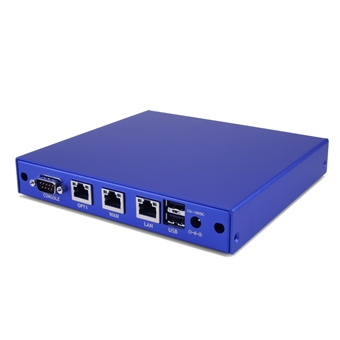
\includegraphics[height=0.3\textheight]{imagens/netgate.jpg}
		\caption{Netgate}
	\end{figure}
	
	DELL
	\begin{figure}
		\centering
		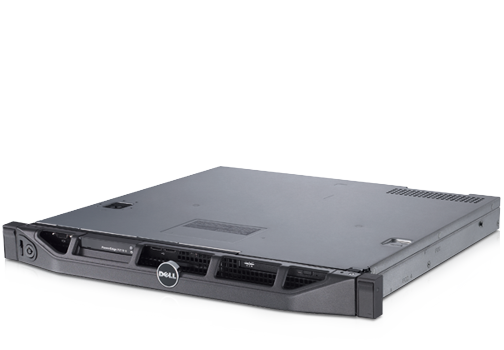
\includegraphics[height=0.3\textheight]{imagens/dell.png}
		\caption{Dell}
	\end{figure}

\end{frame}

%------------------------------------------------

\subsection{Analogia do castelo}


